\section{Match-Level Parameters}
\label{sec:match_level_parameters}

Beyond team-specific strength parameters, the P7 model includes two match-level parameters that capture important structural features of football: home effect ($\nu$) and a common effect parameter on both teams' goal rates ($\eta$).
This section analyses the posterior distributions of these parameters across the 2020--2025 \textit{Brasileirão} seasons.

\subsection{Home Effect}
\label{subsec:home_effect}

The home effect is a well-documented phenomenon in football, where teams playing at their own stadium tend to perform better due to factors such as crowd support, familiarity with the pitch, and reduced travel fatigue \cite{pollard_1986}.
In the P7 model, this effect is captured by the parameter $\nu$, which adds a constant bonus to the log-expected goals of the home team.
The multiplicative effect on expected goals is given by $\exp(\nu)$.
For example, a value of $\nu = 0.30$ implies that the home team is expected to score $\exp(0.30) \approx 1.35$ times more goals than if playing away, holding all other factors constant, i.e., playing against the same team but as an away team.

Figure~\ref{fig:home_effect} shows the posterior distributions of $\nu$ across the analysed seasons.
The 2020 season, played without spectators due to the COVID-19 pandemic from August 2020 through February 2021, exhibits a median $\nu = 0.273$ ($\exp(\nu) \approx 1.31$).
Studies of European leagues during the same period reported substantial reductions in home advantage during closed-door matches \cite{fischer_2021, sors_2021, benz_2023}.
However, this effect is not clearly observed in the \textit{Brasileirão} data: the 2020 estimate is similar to 2023 ($\nu = 0.281$), a season played under normal conditions, and the posterior distributions overlap considerably.
This suggests that crowd presence may not be the dominant driver of home advantage in Brazilian football.
Alternatively, factors such as differences in stadium infrastructure, travel distances, or tactical adaptations, may have compensated for the absence of supporters.

Table~\ref{tab:match_params} summarises the posterior statistics for both match-level parameters across all seasons.

\begin{figure}[htbp]
    \centering
    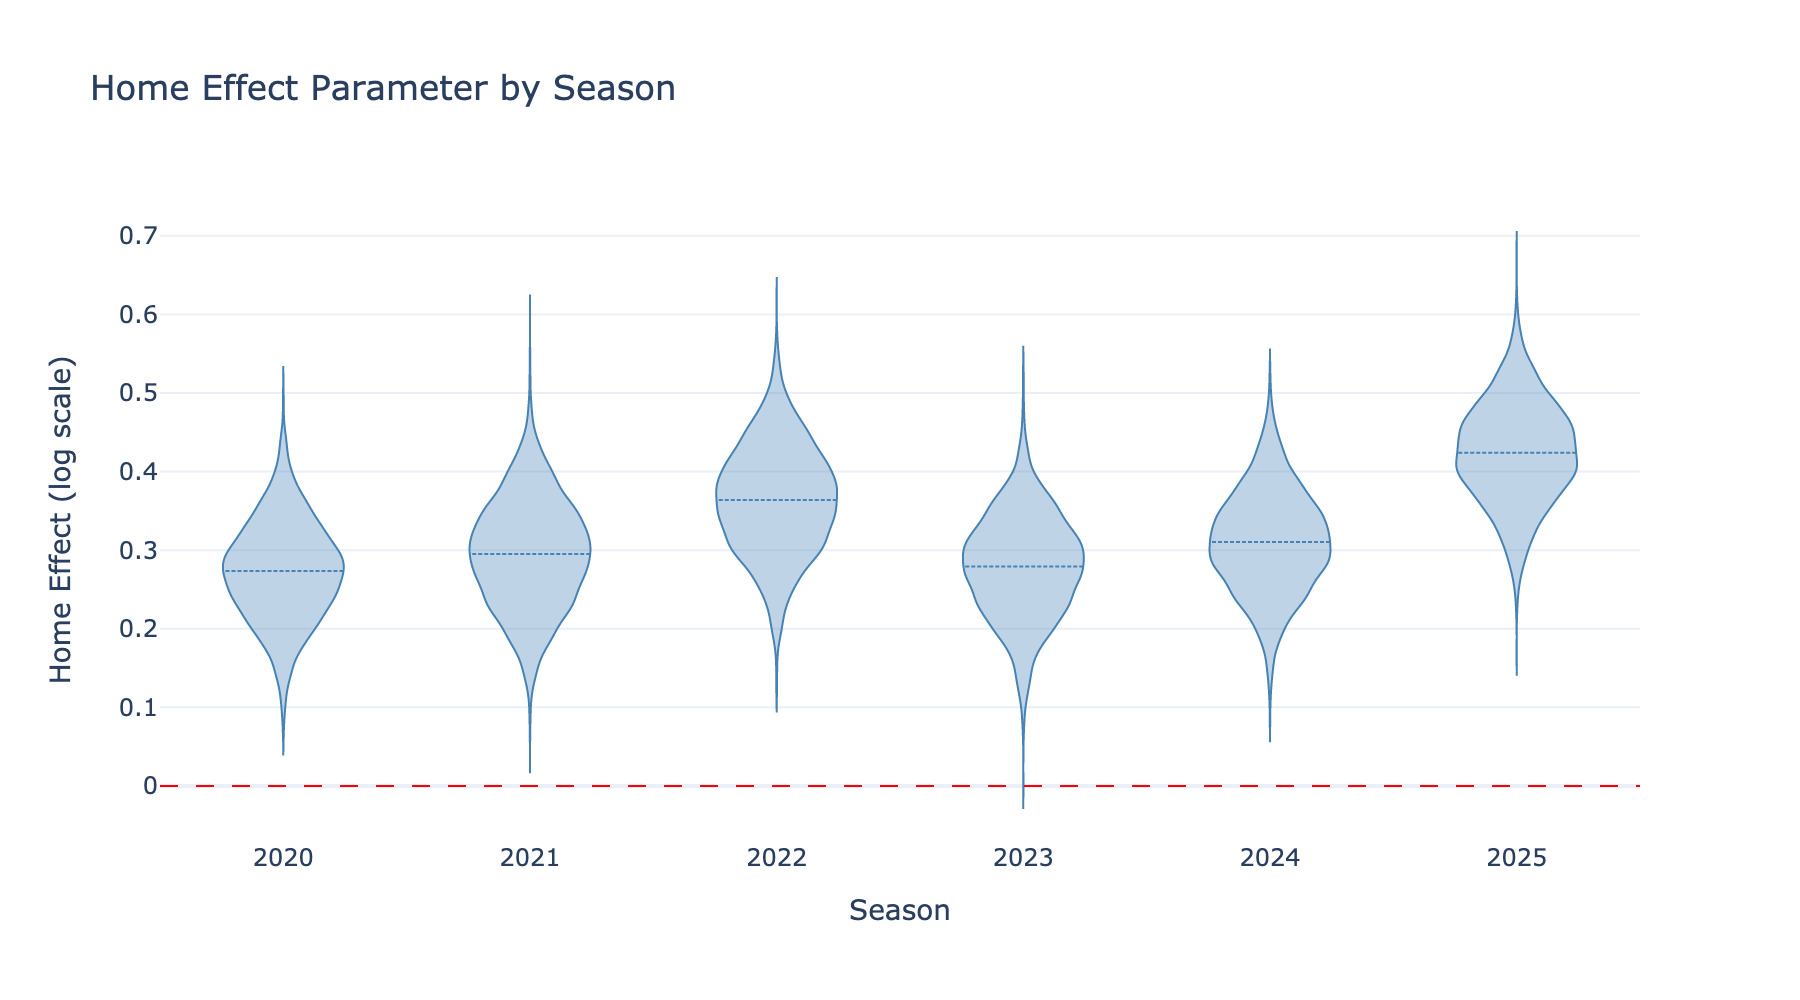
\includegraphics[width=0.9\textwidth]{figures/home_effect_comparison.png}
    \caption{
        \textbf{Posterior distributions of the home effect parameter ($\nu$) across seasons}.
        Each violin plot shows the posterior distribution estimated from 4,000 MCMC samples.
        The dashed horizontal line at zero represents no home effect.
        Higher values indicate stronger home advantage.
    }
    \label{fig:home_effect}
\end{figure}

\subsection{Common Effect on Goals}
\label{subsec:common_effect}

The common effect parameter $\eta$ captures deviations in total goals scored from what would be expected based on team strengths alone.
In the P7 model, $\eta$ affects both teams' expected goals symmetrically.
Positive values indicate that matches tend to produce more goals, while negative values suggest fewer goals than predicted by team quality differences.

Figure~\ref{fig:common_effect_strength} reveals that $\eta$ fluctuates around zero across seasons, with both positive and negative values observed.
The 2020 and 2023 seasons exhibit slightly positive median values ($\eta \approx 0.03$), corresponding to $\exp(\eta) \approx 1.03$, i.e., approximately 3\% more goals than expected.
In contrast, 2021 shows the most negative value (median $\eta = -0.096$, corresponding to $\exp(\eta) \approx 0.91$), i.e., roughly 9\% fewer goals than predicted by team strengths.

These variations may reflect changes in tactical approaches, referee behaviour, or overall league competitiveness.
A negative $\eta$ could indicate a more defensive league style or greater parity among teams, leading to tighter, lower-scoring matches.
The near-zero values observed in most seasons suggest that the team strength parameters already capture the primary drivers of goal-scoring, with $\eta$ making only modest adjustments.
This hypothesis is supported by the fact that the results of the models with common effect are very similar to the results of their counterparts without common effect.

\begin{figure}[htbp]
    \centering
    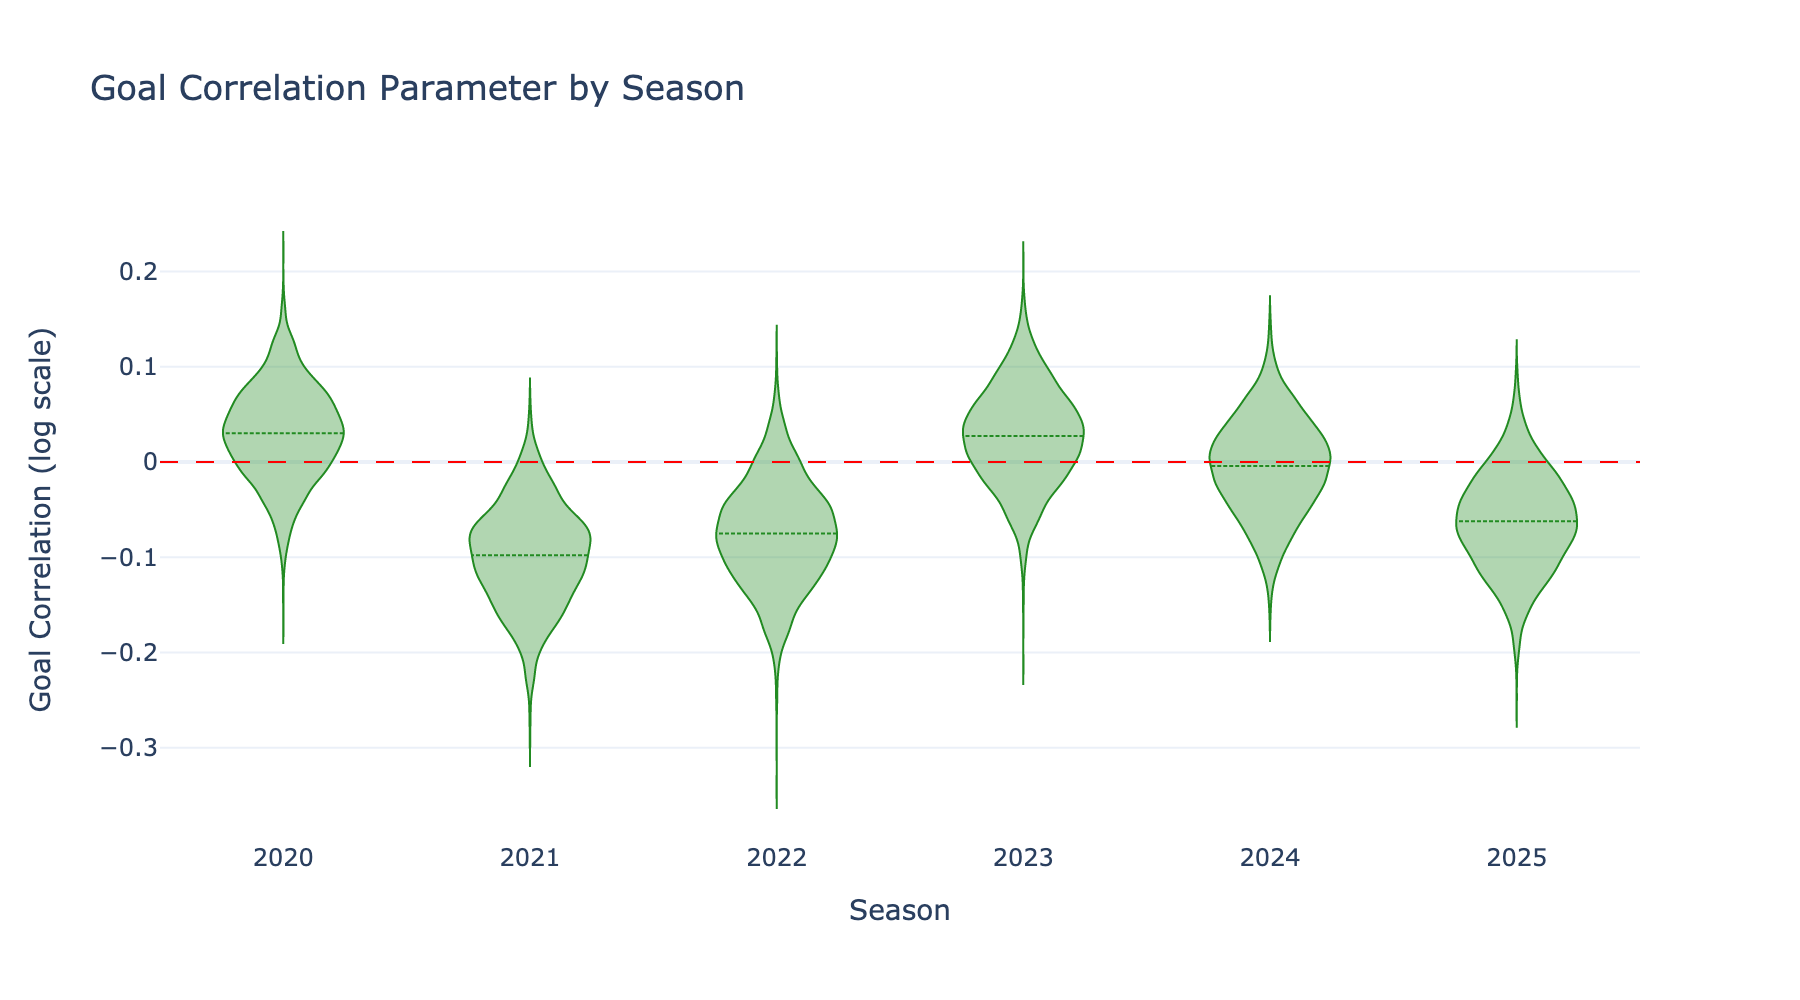
\includegraphics[width=0.9\textwidth]{figures/correlation_strength_comparison.png}
    \caption{
        \textbf{Posterior distributions of the common effect parameter ($\eta$) across seasons}.
        Each violin plot shows the posterior distribution estimated from 4,000 MCMC samples.
        The dashed horizontal line at zero represents no systematic deviation from expected goals.
        Positive values indicate higher-scoring matches; negative values indicate lower-scoring matches.
    }
    \label{fig:common_effect_strength}
\end{figure}

\begin{table}[htbp]
    \centering
    \begin{tabular}{lcccc}
        \toprule
        Season & $\nu$ & $\exp(\nu)$ & $\eta$ & $\exp(\eta)$ \\
        \midrule
        2020 & 0.273 (0.147, 0.402) & 1.31 & 0.031 (-0.069, 0.127) & 1.03 \\
        2021 & 0.296 (0.162, 0.430) & 1.34 & -0.096 (-0.204, 0.004) & 0.91 \\
        2022 & 0.365 (0.226, 0.497) & 1.44 & -0.075 (-0.182, 0.035) & 0.93 \\
        2023 & 0.281 (0.142, 0.404) & 1.32 & 0.028 (-0.071, 0.126) & 1.03 \\
        2024 & 0.310 (0.185, 0.441) & 1.36 & -0.003 (-0.105, 0.091) & 1.0 \\
        2025 & 0.425 (0.293, 0.548) & 1.53 & -0.062 (-0.162, 0.039) & 0.94 \\
        \bottomrule
    \end{tabular}
    \caption{
        \textbf{Summary statistics for match-level parameters by season}.
        Values shown are posterior medians with 2.5th and 97.5th percentiles in parentheses.
    }
    \label{tab:match_params}
\end{table}
